\documentclass[11pt,a4paper]{article}

\usepackage[utf8]{inputenc}
\usepackage[spanish]{babel}
\usepackage{amsmath}
\usepackage{amsfonts}
\usepackage{amssymb}
\usepackage{makeidx}
\usepackage{graphicx}
\usepackage{lmodern}
\usepackage{kpfonts}
\usepackage{wrapfig}
\usepackage{caption}
\usepackage{subcaption}
\usepackage{booktabs}
\usepackage[nottoc,numbib]{tocbibind} %agrega la bibliografia al índice.
\usepackage[font={small,it}]{caption}
%\usepackage{fourier}
\usepackage[left=2cm,right=2cm,top=2cm,bottom=2cm,headheight=13.6pt]{geometry}
\usepackage{fancyhdr}
\usepackage{multirow}
\pagestyle{fancy}


%Para los gráficos en general, con las tablas...¡Ja!, arreglate.
%\begin{figure}[h!]
%\centering
%\includegraphics[width=0.7\textwidth]{} %nombre de la imagen, incluirla en el mismo directorio que este archivo.
%\caption*{} %rótulo, el asterico elimina la numeración automática. 
%\label{fig:} % para luego referirse con \ref{fig:}
%\end{figure}


\begin{document}


%%%%%%%%%%%%%%%%%%%%%%%%%%%%%%%%%%%%%%%%%%%%%%%%%%%%%%%%%%%%%%%%%%%%%%%%%%%%%%%%%%%%%%%%%%%%%%%%%%%%%%%%%%%%%%%%%%%%%%%%%%%%%%%%%
% 	TÍTULO
%%%%%%%%%%%%%%%%%%%%%%%%%%%%%%%%%%%%%%%%%%%%%%%%%%%%%%%%%%%%%%%%%%%%%%%%%%%%%%%%%%%%%%%%%%%%%%%%%%%%%%%%%%%%%%%%%%%%%%%%%%%%%%%%%

%%%%%%%%%%%%%%%%%%%%%%%%%%%%%%%%%%%%%%%%%
% University Assignment Title Page 
% LaTeX Template
% Version 1.0 (27/12/12)
%
% This template has been downloaded from:
% http://www.LaTeXTemplates.com
%
% Original author:
% WikiBooks (http://en.wikibooks.org/wiki/LaTeX/Title_Creation)
%
% License:
% CC BY-NC-SA 3.0 (http://creativecommons.org/licenses/by-nc-sa/3.0/)
% 
% Instructions for using this template:
% This title page is capable of being compiled as is. This is not useful for 
% including it in another document. To do this, you have two options: 
%
% 1) Copy/paste everything between \begin{document} and \end{document} 
% starting at \begin{titlepage} and paste this into another LaTeX file where you 
% want your title page.
% OR
% 2) Remove everything outside the \begin{titlepage} and \end{titlepage} and 
% move this file to the same directory as the LaTeX file you wish to add it to. 
% Then add \input{./title_page_1.tex} to your LaTeX file where you want your
% title page.
%
%%%%%%%%%%%%%%%%%%%%%%%%%%%%%%%%%%%%%%%%%

%----------------------------------------------------------------------------------------
%	PACKAGES AND OTHER DOCUMENT CONFIGURATIONS
%----------------------------------------------------------------------------------------

%\documentclass[12pt]{article}
%\usepackage[utf8]{inputenc}
%\usepackage[spanish]{babel}
%\begin{document}

\begin{titlepage}

\newcommand{\HRule}{\rule{\linewidth}{0.5mm}} % Defines a new command for the horizontal lines, change thickness here

\center % Center everything on the page
 
%----------------------------------------------------------------------------------------
%	HEADING SECTIONS
%----------------------------------------------------------------------------------------

\textsc{\Huge Universidad de Buenos Aires}\\[0.5cm]
\textsc{\LARGE Facultad de Ciencias Exactas y Naturales}\\[0.5cm] % Name of your university/college
\textsc{\Large Departamento de Física}\\[0.25cm] % Major heading such as course name

\begin{figure}[h]
  \centering
  
\includegraphics[scale=0.15]{Logo_DF}
  \\[0.5cm]
\end{figure}

\textsc{\large Laboratorio 3}\\[0.25cm] % Minor heading such as course title

%----------------------------------------------------------------------------------------
%	TITLE SECTION
%----------------------------------------------------------------------------------------

\HRule \\[0.4cm]
{ \huge \bfseries Transitorio y tiempo caracteristico de circuitos}\\[0.2cm] % Title of your document
\HRule \\[1cm]
 
%----------------------------------------------------------------------------------------
%	AUTHOR SECTION
%----------------------------------------------------------------------------------------

\begin{minipage}{0.4\textwidth}
\begin{center} \large
\emph{Autores:}\\
\textsc{Andreu}, Gonzalo\\ % Your name
\textsc{Malpartida}, Bryan\\ % Your name
\textsc{Pugliese}, Facundo\\ % Your name


\end{center}
\end{minipage}
~ \\[1.25cm]
%\begin{minipage}{0.4\textwidth}
%\begin{flushright} \large
%\emph{Supervisor:} \\
%Dr. James \textsc{Smith} % Supervisor's Name
%\end{flushright}
%\end{minipage}\\[4cm]

% If you don't want a supervisor, uncomment the two lines below and remove the section above
%\Large \emph{Author:}\\
%John \textsc{Smith}\\[3cm] % Your name

%----------------------------------------------------------------------------------------
%	DATE SECTION
%----------------------------------------------------------------------------------------

%\vspace{\fill}


{\large 17 de Febrero de 2016}\\[1.75cm] % Date, change the \today to a set date if you want to be precise

%----------------------------------------------------------------------------------------
%	SUMMARY SECTION: No más de 15 renglones, no te zarpes
%----------------------------------------------------------------------------------------

\begin{center}
\large{\textbf{Resumen}}

\small{El objetivo del siguiente trabajo fue caracterizar circuitos RC, RL y RCL. 

Para los dos primeros casos, los circuitos RC y RL, se buscó determinar el tiempos característico de cada uno variando los parámetros de cada sistema. Ademas de poder observar los fenómenos particulares en estos sistemas, como la carga y descarga del capacitor y la disminución de la corriente debido a la inductancia, utilizando una fuente de alimentación que emitía señales cuadradas y osciloscopio como instrumento de medición.

Por otro lado, el estudio del circuito RCL se centró en la observación de los comportamientos que tiene el mismo para distintos parámetros del sistema. Para ellos se obtenían teóricamente los valores necesarios de cada parámetro para luego $settear$ los elementos del circuito y comprobar que la evolución del sistema cumpliese el modelo teórico. Dichas observaciones se obtuvieron nuevamente utilizando una fuente de señal cuadrada y un osciloscopio.

Finalmente, el método resulto eficiente a la hora de comprobar las ecuaciones referidas al circuito RC y, en menor medida, al circuito RL. En el caso del circuito RCL, pudieron analizarse los casos extremos de comportamiento, pero no el comportamiento borde debido a lo fino del mismo.} % ACA VA EL RESUMEN

\end{center}


%----------------------------------------------------------------------------------------
%	LOGO SECTION
%----------------------------------------------------------------------------------------

%\includegraphics{Logo}\\[1cm] % Include a department/university logo - this will require the graphicx package
 
%----------------------------------------------------------------------------------------

\vfill % Fill the rest of the page with whitespace

\end{titlepage}
%\end{document} %incluir en el mismo directorio que este archivo. Equivalente a un copiar-pegar, nada de andar diciendo \begin{document} en la portada. Dejar el nombre de Caratula a la caratula.

%%%%%%%%%%%%%%%%%%%%%%%%%%%%%%%%%%%%%%%%%%%%%%%%%%%%%%%%%%%%%%%%%%%%%%%%%%%%%%%%%%%%%%%%%%%%%%%%%%%%%%%%%%%%%%%%%%%%%%%%%%%%%%%%%
% 	ENCABEZADO Y PIE DE PÁGINA.
%%%%%%%%%%%%%%%%%%%%%%%%%%%%%%%%%%%%%%%%%%%%%%%%%%%%%%%%%%%%%%%%%%%%%%%%%%%%%%%%%%%%%%%%%%%%%%%%%%%%%%%%%%%%%%%%%%%%%%%%%%%%%%%%%

\lhead{}
\chead{}
\rhead{Laboratorio 3}
\lfoot{}
\cfoot{}
\rfoot{\thepage}
\renewcommand{\headrulewidth}{1pt}
\renewcommand{\footrulewidth}{1pt}


%%%%%%%%%%%%%%%%%%%%%%%%%%%%%%%%%%%%%%%%%%%%%%%%%%%%%%%%%%%%%%%%%%%%%%%%%%%%%%%%%%%%%%%%%%%%%%%%%%%%%%%%%%%%%%%%%%%%%%%%%%%%%%%
% Página en blanco. Cita, agradecimiento, dedicación, lo que sea pero que sea algo.
%%%%%%%%%%%%%%%%%%%%%%%%%%%%%%%%%%%%%%%%%%%%%%%%%%%%%%%%%%%%%%%%%%%%%%%%%%%%%%%%%%%%%%%%%%%%%%%%%%%%%%%%%%%%%%%%%%%%%%%%%%%%%%%


%%%%%%%%%%%%%%%%%%%%%%%%%%%%%%%%%%%%%%%%%%%%%%%%%%%%%%%%%%%%%%%%%%%%%%%%%%%%%%%%%%%%%%%%%%%%%%%%%%%%%%%%%%%%%%%%%%%%%%%%%%%%%%%%%
% 	ÍNDICE
%%%%%%%%%%%%%%%%%%%%%%%%%%%%%%%%%%%%%%%%%%%%%%%%%%%%%%%%%%%%%%%%%%%%%%%%%%%%%%%%%%%%%%%%%%%%%%%%%%%%%%%%%%%%%%%%%%%%%%%%%%%%%%%%%

%\tableofcontents %compilar dos o tres veces para verlo bien. ¡Todo un índice en unas cuantas letras!
%\newpage

%%%%%%%%%%%%%%%%%%%%%%%%%%%%%%%%%%%%%%%%%%%%%%%%%%%%%%%%%%%%%%%%%%%%%%%%%%%%%%%%%%%%%%%%%%%%%%%%%%%%%%%%%%%%%%%%%%%%%%%%%%%%%%%
% 1. RESUMEN
%%%%%%%%%%%%%%%%%%%%%%%%%%%%%%%%%%%%%%%%%%%%%%%%%%%%%%%%%%%%%%%%%%%%%%%%%%%%%%%%%%%%%%%%%%%%%%%%%%%%%%%%%%%%%%%%%%%%%%%%%%%%%%%

%\section{Resumen}
%\label{sec:resumen}



%%%%%%%%%%%%%%%%%%%%%%%%%%%%%%%%%%%%%%%%%%%%%%%%%%%%%%%%%%%%%%%%%%%%%%%%%%%%%%%%%%%%%%%%%%%%%%%%%%%%%%%%%%%%%%%%%%%%%%%%%%%%%%%
% 2. INTRODUCCIÓN: ecuaciones aquí, luego se las cita.
%%%%%%%%%%%%%%%%%%%%%%%%%%%%%%%%%%%%%%%%%%%%%%%%%%%%%%%%%%%%%%%%%%%%%%%%%%%%%%%%%%%%%%%%%%%%%%%%%%%%%%%%%%%%%%%%%%%%%%%%%%%%%%%

\section{Introducción}\label{sec:intro}



%%%%%%%%%%%%%%%%%%%%%%%%%%%%%%%%%%%%%%%%%%%%%%%%%%%%%%%%%%%%%%%%%%%%%%%%%%%%%%%%%%%%%%%%%%%%%%%%%%%%%%%%%%%%%%%%%%%%%%%%%%%%%%%
% 3. DISPOSITIVO EXPERIMENTAL: armado del modelo, como se midio, consideraciones a la hora de medir.
%%%%%%%%%%%%%%%%%%%%%%%%%%%%%%%%%%%%%%%%%%%%%%%%%%%%%%%%%%%%%%%%%%%%%%%%%%%%%%%%%%%%%%%%%%%%%%%%%%%%%%%%%%%%%%%%%%%%%%%%%%%%%%%

\section{Desarrollo experimental}

Durante esta experiencia se utilizó ,como fuente alterna, un generador de funciones el cual se programo para que generara un diferencia de potencial que variara en el tiempo con la forma $\epsilon = E_{0}cos(\omega t)$, donde $E_{0}$ es la amplitud maxima y en el informe se referira a ella como Amplitud. Este generador es capaz de emitir frecuencias con un error relativo del $0,01\%$ en un rango entre $1\mu Hz$ y $5MHz$ cuyo voltaje pico-pico tiene un error relativo del $1\%$ para el rango de voltaje utilizado ($2V-20V$). Además, se utilizó una capacitancia fija $C = (100,0 \pm 0,2)nF$ y una resistencia variable por décadas cuyo error fue a priori desconocido. Usando un multimetro digital se midieron las resistencias utilizadas junto con su error, que era de la forma $\pm(1\%+2d)$ para el rango de resistencias utilizadas (mayores a $100\Omega$). La resistencia del capacitor resultó despreciable. También, se utilizó una inductancia fija $L = (1.000 \pm 0.002) H$ que poseía una resistencia interna (medida por el multímetro) $R_L = (294 \pm 3) \Omega$.
Finalmente, se utilizó un osciloscopio digital que en sus dos canales de entrada era capaz de medir diferencias de potencial entre las dos terminales que dispone en un rango de 2mV a 5V con un error relativo del $3\%$. A la hora de medir voltaje, fue necesario asegurarse que el cable a tierra del osciloscopio estuvera conectado al cable a tierra el generador de funciones. 



\subsection{Resonancia y Anti-Resonancia}
Durante la experiencia estudió el comportamiento de circuitos RCL sometidos a corrientes con distintas frecuencias. En primer lugar se quiso estudiar el efecto de resonacia, por lo cual se construyó un circuito cerrado que constaba de la fuente $\varepsilon$, la resistencia variable por decadas fijada en un valor $R = (5 \pm 0,05)K\Omega$, una inductancia con un valor $L = (1 \pm 0.002)H$ con una Resistencia $R_{L}= (296\pm 3)\Omega$ que fue despreciada frente al valor de la mencionada anteriormente, y una capacitacia $C = (9.95 \pm 0.07)nF$, conectados en serie como muestra la \textbf{Figura \ref{fig:RCL-Res}}. Cabe destacar que, previamente a la construccion el dispositivo,  se utilizó el multimetro para asegurar la continuidad de todos los cables utilizados, y que esta misma no se viera comprometida por movimientos aleatorios, a fin de poder reducir una fuente de posibles incertezas.

\begin{figure}[h]
\centering
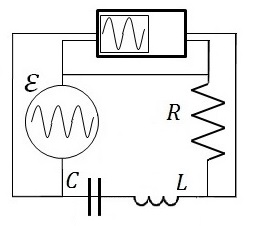
\includegraphics[scale=0.7]{Circuito-RCL-Resonante}
  \caption{Circuito RCL con una fuente sinusoidal capaz de entrar en un estado de resonancia}
  \label{fig:RCL-Res}
\end{figure}

Para medir la diferencia de tension se conectó, en paralelo, un canal del osciloscopio a la resistencia. Se utilizo una llave T para conectar en paralelo a la fuente el segundo canal del osciloscopio, logrando de esta manera, que se desplegaran en la pantalla las dos señales al mismo tiempo y nos diera la posibilidad de medir la diferencia de fase entre las señales. Además, tambien se utilizó la frecuencia de esa segunda señal como \textit(trigger externo) para asegurar una imagen estatica en la pantalla del osciloscopio. Se fijo una Amplitud $E_{0} = (8,00 \pm 0,08)V$, y se fijo una frecuencia. Se tomó nota del desfasaje y de la amplitud calculados por el osciloscopio para la señal de salida y, una ves hecho esto, se varió la frecuencia. Este proceso se itero hasta tener suficientes mediciones como para realizar un grafico. Una vez terminada la adquisicion de datos, se repitio el proceso con un cicuito con los mismos parametros, a excepcion de la Resistencia, a la cual se le cambio el valor a $R = (500 \pm 5)$. Vale la pena aclarar que para este segundo circuito, la resistencia producida por la inductancia no era despreciable y fue tenida en cuenta.

Luego, se estudió el caso de la anti-resonancia, y para esto se diseño un circuito RCL similar al anterior, con la salvedad que en este caso el capacitor se encontraba conectado en paralelo a la inductancia como ilustra la \textbf{Figura \ref{fig:RCL-ARes}}. De la misma forma que en el caso de resonancia, se realizaron dos juegos de ediciones y para ambas se utilizo una inductancia con un valor $L = (1 \pm0.002)H$ y una capacitacia $C = (9.95 \pm 0.07)nF$, la fuente se fijo en una Amplitud $E_{0} = (8,00 \pm 0,08)V$, Y la resistencia tuvo un valor $R = (5 \pm 0,05)K\Omega$ durante la primer medición, y en $R = (1 \pm 0,01)K\Omega$ durante la segunda.

\begin{figure}[h]
\centering
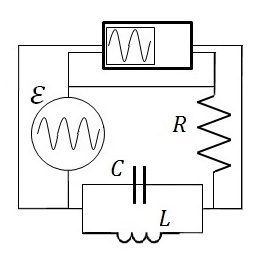
\includegraphics[scale=0.7]{Circuito-RCL-AntiResonante}
  \caption{Circuito RCL con una fuente sinusoidal incapaz de entrar en un estado de resonancia (Anti-Resonante)}
  \label{fig:RCL-ARes}
\end{figure}

De manera analoga al metodo utilizado con el circuito resonante, el osciloscopio se conecto de forma paralela a la resistencia y a la fuente, y se tomaron nota de los desfasajes y amplitudes de la corriente de salida.


\subsection{Filtros}

El objetivo de esta parte fue experimentar con distintos tipos de filtros, para esto se contruyó un cirtuito que costaba de una resistencia $R = (5 \pm 0.05)k\Omega$, una capacitancia $C = (10.00 \pm 0.03)nF$ colocadas y un generador de funciones con una Amplitud $E_{0} = (9.4 \pm 0.2)V$, colocados en serie. Para un primer analisis, se utilizaron como terminales de salida los extremos del Capacitor obteniendo así, un filtro pasa-bajos, como se muestra en la \textbf{figura \ref{fig:RC-PB}}. Cabe destacar, que de la misma manera que se hizo durante los experimentos de resonancia, se aseguro la continuidad de todos los cables a utilizar.

\begin{figure}[h]
\centering
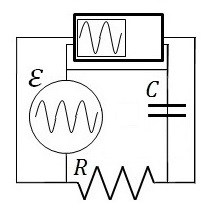
\includegraphics[scale=0.9]{Circuito-RC-Pasa-Bajos}
  \caption{Circuito RC capaz de filtrar corrientes con frecuencias altas, con un osciloscopio conectado en paralelo a la fuente y al capacitor}
  \label{fig:RC-PB}
\end{figure}

Antes de realizar las mediciones se calculo la frecuencia de corte del filtro para asegurar que se relevaran datos que correspondieran tanto a las señales que eran atenuadas como a las que no. Una vez realizada esa salvedad, se utilizo el mismo procedimiento de medicion que se utilizo con el circuito resonante. 

Una vez finalizadas las mediciones sobre el dispositivo, se procedio a ver el caso del filtro Pasa-Altos; para lo cual se cambiaron las terminales de salida, colocandose en los extremos de la resistencia como ilustra la \textbf{figura \ref{fig:RC-PA}}. No se realizaron variaciones en ninguno de los parametros, pero si se cambió la posicion de la descarga a tierra del generador de funciones para que coincidiera con la del osciloscopio.

\begin{figure}[h]
\centering
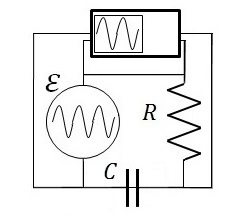
\includegraphics[scale=0.9]{Circuito-RC-Pasa-Altos}
  \caption{Circuito RC capaz de filtrar corrientes con frecuencias bajas, con un osciloscopio conectado en paralelo a la fuente y al capacitor}
  \label{fig:RC-PA}
\end{figure}

El Procedimiento de medicion para este circuito, fue completamente analogo al realizado anteriormente con el circuito Pasa-Bajos. 

Finalmente se procedio a combinar ambos filtros para, de esta menera, formar un pasa-banda como se puede ver en la \textbf{figura \ref{fig:RC-PBD}}. En este caso si se cambiaron los parametros. Se fijarom ambas resistencias en un valor $R = (1 \pm 0.009)k\Omega$ y una capacitancia $C_{1} = (10.02 \pm 0.02)nF$ y una $C_{2} = (100.0 \pm 0.3)nF$. Cabe destacar que estos valores se eligieron de forma tal que la frecuencia de corte del pasabajos sea un orden de magnitud mayor que la del pasa altos y asi poder apreciar la campana de transferencia. 

\begin{figure}[h]
\centering
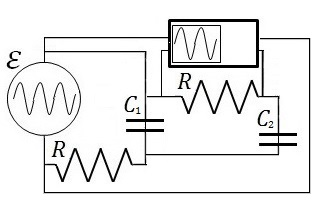
\includegraphics[scale=0.8]{Circuito-RC-Pasa-Banda}
  \caption{Circuito RC capaz de filtrar las corrrientes cuya frecuencia este por fuera del ancho de banda estipulado por los parametros del mismo. Ambas resistencia 
tienen el mismo valor y la capacitancia $c_{1}$ es menor que $c_{2}$}
  \label{fig:RC-PBD}
\end{figure}

Una vez finalizada la construccion del dispositivo, se procedio a medir de la manera detallada anteriormente.


%%%%%%%%%%%%%%%%%%%%%%%%%%%%%%%%%%%%%%%%%%%%%%%%%%%%%%%%%%%%%%%%%%%%%%%%%%%%%%%%%%%%%%%%%%%%%%%%%%%%%%%%%%%%%%%%%%%%%%%%%%%%%%%%
% 4.DISCUSIÓN Y RESULTADOS: todo lo que se obtuvo y explicación. Graficos, tablas.
%%%%%%%%%%%%%%%%%%%%%%%%%%%%%%%%%%%%%%%%%%%%%%%%%%%%%%%%%%%%%%%%%%%%%%%%%%%%%%%%%%%%%%%%%%%%%%%%%%%%%%%%%%%%%%%%%%%%%%%%%%%%%%%%

\section{Resultados}
\label{sec:discusion}



%%%%%%%%%%%%%%%%%%%%%%%%%%%%%%%%%%%%%%%%%%%%%%%%%%%%%%%%%%%%%%%%%%%%%%%%%%%%%%%%%%%%%%%%%%%%%%%%%%%%%%%%%%%%%%%%%%%%%%%%%%%%%%%%
%	CONCLUSIONES
%%%%%%%%%%%%%%%%%%%%%%%%%%%%%%%%%%%%%%%%%%%%%%%%%%%%%%%%%%%%%%%%%%%%%%%%%%%%%%%%%%%%%%%%%%%%%%%%%%%%%%%%%%%%%%%%%%%%%%%%%%%%%%%%

\section{Conclusiones}
\label{sec:conclusiones}




%%%%%%%%%%%%%%%%%%%%%%%%%%%%%%%%%%%%%%%%%%%%%%%%%%%%%%%%%%%%%%%%%%%%%%%%%%%%%%%%%%%%%%%%%%%%%%%%%%%%%%%%%%%%%%%%%%%%%%%%%%%%%%%%%
%	APÉNDICE: esas cosas extras que simplemente no tuvieron lo suficiente como para ganarse una sección propia.
%%%%%%%%%%%%%%%%%%%%%%%%%%%%%%%%%%%%%%%%%%%%%%%%%%%%%%%%%%%%%%%%%%%%%%%%%%%%%%%%%%%%%%%%%%%%%%%%%%%%%%%%%%%%%%%%%%%%%%%%%%%%%%%%%



%%%%%%%%%%%%%%%%%%%%%%%%%%%%%%%%%%%%%%%%%%%%%%%%%%%%%%%%%%%%%%%%%%%%%%%%%%%%%%%%%%%%%%%%%%%%%%%%%%%%%%%%%%%%%%%%%%%%%%%%%%%%%%%%%
%	REFERENCIAS: libros, libros, libros.
%%%%%%%%%%%%%%%%%%%%%%%%%%%%%%%%%%%%%%%%%%%%%%%%%%%%%%%%%%%%%%%%%%%%%%%%%%%%%%%%%%%%%%%%%%%%%%%%%%%%%%%%%%%%%%%%%%%%%%%%%%%%%%%%%

%Ejemplo:
\begin{thebibliography}{1}
 \bibitem{Berkeley} Frank S. Crawford, \textit{Berkeley physics course 3: Ondas}, 1994, Editorial Reverte S.A.
\end{thebibliography}
%Para citar: blablabla \cite{Baird}
 
\end{document}





